\documentclass[11pt]{article}
\usepackage[a4paper, margin=2.5cm]{geometry}
\usepackage[T1]{fontenc}
\usepackage{polski}
\usepackage{babel}
\usepackage{indentfirst}
\usepackage{listings}
\usepackage[colorlinks=true, urlcolor=blue, linkcolor=red]{hyperref}
\usepackage[document]{ragged2e}
\usepackage{graphicx}
\graphicspath{ {.} }
\usepackage[font=small,labelfont=bf]{caption}

\lstset{
	frame=l,
	basicstyle=\ttfamily,
	numbers=left,
	texcl=false,
	tabsize=1,
	breaklines=true,
	postbreak=\mbox{{$\hookrightarrow$}\space}
}

\sloppy

\title{
	\textbf{Architektury głębokiego uczenia}\\
	Analiza użycia \texttt{FaceNet} do rozpoznawania ras psów}

    \author{
        Bartosz Leśniewski, 184783
        \and
        Jakub Kuczys, 184***
        \and
        Wojciech Panfil, 184657
      }

\date{5 czerwca 2024}

\begin{document}
    \maketitle

    \justify

    \section{Wprowadzenie i analiza problemu badawczego}

    Autorzy niniejszego sprawozdania postanowili podjąć się analizy systemu \texttt{FaceNet} opisanego w artykule
    \href{https://arxiv.org/abs/1503.03832}{\texttt{FaceNet}: A Unified Embedding for Face Recognition and Clustering}
    w którym autorzy - Florian Schroff, Dmitry Kalenichenko oraz James Philbin pracujący w \texttt{Google} podjęli się próby wykonania postępu
    w dziedzinie rozpoznawania twarzy. Jak wspominają sami autorzy, pomimo znaczących ostatnich postępów w tej dziedzienie
    skuteczne wdrażanie weryfikacji i rozpoznawania twarzy na dużą skalę stanowi poważne wyzwanie. 
    \begin{center}
    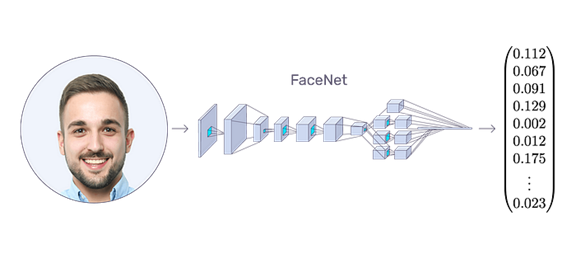
\includegraphics{facenet_arch.png}
    \captionof{figure}{Zasada działania FaceNet}
    \end{center}

    W tym momencie warto przypomnieć kroki, na jakie dzieli się rozpoznawanie twarzy.
    \begin{enumerate}
        \item Wykrywanie twarzy
        \item Ekstrakcja cech (wyodrębnienie wybranych cech obrazu)
        \item Klasyfikacja twarzy (na podstawie cech)
    \end{enumerate}
    System FaceNet operuje w drugim oraz trzecim etapie, co zostanie przedstawione w dalszej części opisu.

    Wewnętrznie, system ten wykorzystuje głęboką sieć konwolucyjną, wyszkoloną do bezpośredniej optymalizacji
    osadzenia twarzy w przestrzeni, co stanowi różnicę w porównaniu do uprzednich podejść do tego problemu. Warto tutaj zaznaczyć, że autorzy
    nie definiują architektury modelu używanego wewnątrz systemu. W artykule wykorzystane i zestawione zostały dwie - \texttt{Zeiler\&Fergus} oraz \texttt{InceptionResnetV1}. 
    Do trenowania, wykorzystywana jest trójkowa funkcja straty (triplet loss function) do której potrzebne są trzy
    twarze - dwie pasujące (anchor i positive) oraz jedna nie pasująca (negative).
    Celem treningu jest zatem minimalizowanie odległości pomiędzy wektorami pasujących do siebie twarzy, a maksymalizacja odległości
    do wektora odpowiadającemu niepasującej twarzy.

    \begin{center}
        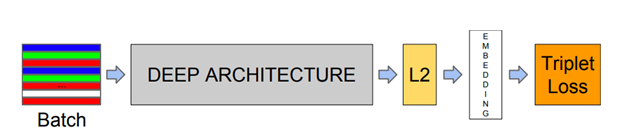
\includegraphics{architecture.png}
        \captionof{figure}{Architektura systemu FaceNet}
    \end{center}

    Zaletą takiego podejścia jest znacznie większa wydajność pamięciowa - na twarz potrzeba jedynie $128$ bajtów (FaceNet uczy się odwzorowywać
    twarz (embedding) na wektor w $128$ wymiarowej przestrzeni euklidesowej).

    Autorom tego systemu, na popularnym zbiorze danych "Labeled Faces in The Wild" udało się uzyskać wynik $99.64\%$ dokładności,
    co wyznaczało nowy rekord. Oznaczało to, że system obniżył poziom błędu w porównaniu do najlepszego wówczas opublikowanego wyniku o $30\%$.

    Do rozpoznawania osoby obrazu wykorzystuje się odwzorowanie na wektor. Po odzworowaniu należy obliczyć odległość pomiędzy tym, a innym znanym odzworowaniem twarzy danej osoby.
    Jeśli ta odległość jest odpowiednio mała uznaje się, że obraz zawiera twarz danej osoby.
    \begin{center}
    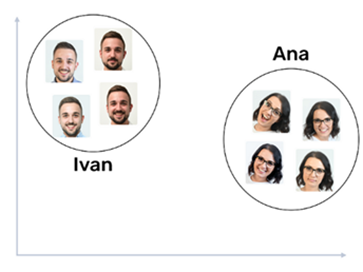
\includegraphics{grouped_faces.png}
    \captionof{figure}{Podobne twarze zgrupowane w przestrzeni euklidesowej}
    \end{center}

    Proces uczenia modelu dzieli się na kilka etapów. Początkowo generowane są losowe wektory dla każdego obrazu - są one losow rozrzucone w układzie współrzędnych.
    Następnie losowo wybierany jest obraz służący jako kotwica, a dalej obraz przedstawiający tą samą osobę co kotwica (positive example). Następnie wybierany jest "negative example",
    czyli losowy obraz innej osoby niż na pozostałych dwóch fotografiach. Uczenie, jak wcześniej wspomniano, polega na takim dostosowywaniu parametrów modelu, aby positive znajdował się blisko anchor,
    a jednocześnie negative daleko - trójkowa funkcja straty.

    \begin{center}
        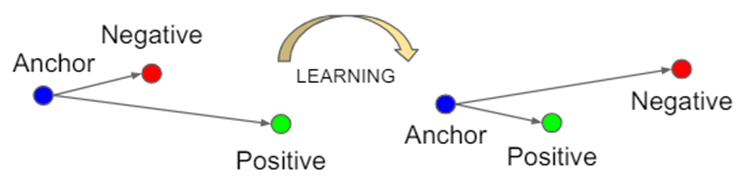
\includegraphics{triplet.png}
        \captionof{figure}{Zasada działania trójkowej funkcji straty}
    \end{center}

    Celem niniejszego projektu była próba odtworzenia eksperymentu przeprowadzonego przez inżynierów Google'a, a następnie przetestowanie
    jego możliwości na znalezionym zestawie danych - \href{https://www.kaggle.com/datasets/wutheringwang/dog-face-recognition}{dog-face-recognition}
    udostępnionym w serwisie Kaggle celem sprawdzenia jak model nauczony na ludzkich twarzach sprawdzi się na innych obiektach.
    Dodatkowo, autorzy zdecydowali się spróbować dotrenować model na mordach psów, celem sprawdzenia skuteczności
    w rozpoznawaniu po kilkunastu epokach treningowych.

    Warto wspomnieć, że istnieje wiele implementacji FaceNet dostępnych w internecie. Najbardziej popularną jest \href{https://github.com/davidsandberg/facenet}{napisana przez David'a Sandberg'a}
    w Tensorflow, natomiast nie jest ona aktualizowana od ponad 6 lat. Do naszych eksperymentów zdecydowaliśmy się wykorzystać \href{https://github.com/timesler/facenet-pytorch}{gotową implementację FaceNet stworzoną przez Tim'a Esler'a},
    która opiera się na framework'u \texttt{PyTorch}, ponadto jest bieżąco utrzymywana.
    Zawiera ona nie tylko samą implementację, ale także dwa przetrenowane modele - jeden na zbiorze \href{https://paperswithcode.com/dataset/vggface2-1}{vggface2}, 
    a drugi na zbiorze \href{https://www.kaggle.com/datasets/debarghamitraroy/casia-webface}{CasiaWebface}. Dodatkowo, zawiera ona implementację MCTCNN, który pomocny jest w wykrywaniu
    twarzy, a następnie umożliwia docięcie zdjęcia do określonych wymiarów, tak aby była na nim wykryta twarz.

    \section{Metodologia}
    W opisie metryk wykorzystane zostaną następujące oznaczenia:
    \begin{enumerate}
        \item $D(x_i, y_i)$ - odległość euklidesowa
        \item $P_{same}$ - wszystkie pary twarzy tego samego podmiotu
        \item $P_{diff}$ - wszystkie pary twarzy różnych podmiotów
    \end{enumerate}

    Skuteczność mierzona będzie za pomocą następujących metryk:
    \begin{enumerate}
        \item Poprawne akceptacje dla progu $d$: $TA(d) = {(i, j) \in P_{same}}$ dla $D(x_i, y_i) \leq d $
        \item Fałszywe akceptacje dla progu $d$: $FA(d) = {(i, j) \in P_{diff}}$ dla $D(x_i, y_i) \leq d $
        \item Wskaźnik dokładności (skuteczności) rozpoznawania $ACC(d) = \frac{TA(d) + (P_{diff} - FA(d))}{P_{same} + P_{diff}}$
        % \item Wskaźnik (odsetek) poprawnych akceptacji (dokładności): $VAL(d) = \frac{TA(d)}{P_{same}}$
        % \item Wskaźnik (odsetek) nieprawidłowych akceptacji (dokładności): $FAR(d) = \frac{FA(d)}{P_{diff}}$
    \end{enumerate}

    W dalszej części sprawozdania używana będzie wyłącznie ostatnia metryka, która jest złożeniem dwóch pierwszych.

    W pierwszej części eksperymentu powtórzony został eksperyment zawarty w artykule, aby potwierdzić poprawność konfiguracji środowiska.
    Następnie zostanie przeprowadzona ewaluacja modelu na zbiorze \texttt{dog-face-recognition}, następnie uruchomione zostanie uczenie na tym zbiorze,
    aby następnie ponownie sprawdzić jak radzi sobie model po treningu na tym samym zbiorze.

    \section{Wyniki eksperymentów, dyskusja i przyszła praca}

    \subsection{Reprodukcja eksperymentu zawartego w artykule - baseline}
    Pierwszy elementem eksperymentu było uruchomienie gotowego modelu \texttt{vggface2} na wspominanym wcześniej zbiorze \texttt{LFW}.
    W tym celu wykorzystany został \href{https://github.com/timesler/facenet-pytorch/blob/master/examples/lfw_evaluate.ipynb}{gotowy przykład dostępny w używanym repozytorium}.
    Program rozpoczyna od załadowania zdjęć wskazanego dataset, a następnie wykrywanie twarzy z pomocą MTCNN oraz ich docięcie do formatu 160x160 pikseli.
    Do ewaluacji tak przygotowanych obrazów wymagany był dodatkowo plik z parami obrazów zwany dalej \texttt{pairs.txt}, który zawierał wygenerowane pary obrazów pasujących oraz niepasujących na podstawie zdjęć zawartych
    w zbiorze danych. Do jego wygenerowania została wykorzystana \href{https://github.com/VictorZhang2014/facenet/blob/master/mydata/generate_pairs.py}{gotowa implementacja generatora}.
    Poprawność przytoczonego narzędzia została również później sprawdzona z \href{vis-www.cs.umass.edu/lfw/pairs.txt}{plikiem udostępnianym ze zbiorem LFW}, co dało analogiczne rezultaty.
    Załadowane zdjęcia zostały przekazywane parami do modelu celem odwzorowania na wektor w przestrzeni euklidesowej.
    W kolejnej części, odwzorowania zostały poddane ocenie w kolejności i ustawieniu zdefiniowanym w pliku par. Odległość pomiędzy poszczególnymi była liczona metryką euklidesową.
    Ocena polegała na walidacji metodą K-fold. Jest to statystyczna metoda pozwalająca na porównywywanie i selekcję modelu dla danego problemu. Pozwala na oceną "umiejętności" modelu na danych danych.
    Na początku liczony był dystans pomiędzy dwoma odwzorowaniami twarzy. Następnie dobierane były wartości graniczne (thresholds), które później służyły do określenia czy dana odległość przykłada się na identyczność twarzy,
    czy na ich odmienność.
    \begin{lstlisting}[language=Python, caption={Implementacja w języku Python},captionpos=b]
    \end{lstlisting}

    Lokalne uruchomienie eksperymentu dało rezultat $99.28\%$ dokładności, co jest znacząco bliskie uzyskanej przez autorów artykułu wartości $99.64$\%.
    Dzięki temu autorzy potwierdzili, że ich środowisko jest działające, w związku z czym przeszli do kolejnej części eksperymentu.

    \subsection{Ewaluacja na zbiorze \texttt{dog-face-recognition}}

    Kolejnym krokiem była ewaluacja na zbiorze \texttt{dog-face-recognition}. W tym celu wykorzystany został ponownie przykład przytoczony w poprzedniej sekcji, tym razem na innym zbiorze.

    \subsection{Trening na zbiorze \texttt{dog-face-recognition}}

    \subsection{Ponowna ewaluacja po treningu}

    \subsection{Przyszła praca}
    
    \section{Bibliografia}
    \begin{enumerate}
        \item \href{https://arxiv.org/abs/1503.03832}{FaceNet: A Unified Embedding for Face Recognition and Clustering}
        \item \href{https://en.wikipedia.org/wiki/FaceNet}{FaceNet basic information}
        \item \href{https://arxiv.org/abs/1604.02878}{Joint Face Detection and Alignment using Multi-task Cascaded Convolutional Networks}
        \item \href{https://medium.com/@culuma/face-recognition-with-facenet-and-mtcnn-11e77240adb6}{Face Recognition with FaceNet and MTCNN}
        \item \href{https://www.researchgate.net/profile/De-Rosal-Ignatius-Moses-Setiadi/publication/346417651_Study_Analysis_of_Human_Face_Recognition_using_Principal_Component_Analysis/links/605a0218458515e83467c633/Study-Analysis-of-Human-Face-Recognition-using-Principal-Component-Analysis.pdf}{Face Recognition using FaceNet Survey, Performance Test, and Comparison}
    \end{enumerate}
\end{document}